\chapter{TINJAUAN PUSTAKA}
% contoh opsi lain Bab 2
%\chapter{DASAR TEORI}


\section{Penelitian Terdahulu}
\begin{table}[h]
    \centering
    \caption{Penelitian Terdahulu}
    \begin{tabular}{c c c c}
        \hline
        \textbf{Author(s)} & \textbf{Metode} & \textbf{Hasil Penelitian} \\ \hline
        Hao Xue et al.\cite{Xue_2021} & Transformer-CP & 
        \begin{minipage}[t]{0.5\textwidth}
            \raggedright
            Model berbasis Transformer dengan Constrantive Pre-training yang menggunakan random masking dengan fitur ekstraksi MFCC mendapatkan akurasi 87,74\% pada data suara batuk pasien covid-19
        \end{minipage} \\ \hline
        Li Xiao et al.\cite{xiao2024lungadapter} & LungAdapter &
        \begin{minipage}[t]{0.5\textwidth}
            \raggedright
            Metode ini menggabungkan blok \textit{trainable} ke dalam model AST yang telah dilatih sebelumnya, yang memungkinkan ekstraksi informasi penting tentang klasifikasi suara paru-paru dari model. Model mencapai kinerja yang baik dengan score 62,40\%.
        \end{minipage}\\ \hline
        Victor Basu et al.\cite{9080747} & GRU, MFCC &
        \begin{minipage}[t]{0.5\textwidth}
            \raggedright
            Lapisan GRU (gated recurrent unit) digunakan untuk memecahkan masalah gradien yang hilang dalam RNN standar. Akurasi: 95,67 $\pm$ 0,77\%.
        \end{minipage}\\ \hline
    \end{tabular}
    \label{tab:previous_research}
\end{table}

\section{Penyakit Paru-paru}
Jenis penyakit paru-paru yang diamati pada penelitian ini terdapat pada \ref{subsection:copd} dan \ref{subsection:asma}.
\subsection{\textit{Chronic obstructive pulmonary disease} (COPD)}
\label{subsection:copd}
\textit{Chronic Obstructive Pulmonary Disease} (COPD) memiliki berbagai gejala yang sering kali dapat disalahartikan sebagai kondisi pernapasan lainnya, sehingga mempersulit diagnosis dan penanganannya. Gejala utamanya meliputi batuk kronis \cite{PMID:31710455}, dispnea \cite{singh2017chronic}, dan produksi sputum \cite{mannino2001chronic}, yang tumpang tindih dengan kondisi seperti asma dan bronkitis.
\subsection{Asma}
\label{subsection:asma}
Asma adalah suatu kondisi pernapasan kronis yang ditandai dengan gejala yang bervariasi, terutama mengi, batuk, dada terasa sesak, dan dispnea yang intensitas dan frekuensinya dapat berfluktuasi \cite{PMID:35143150}. Gejala-gejala ini sering kali timbul dari pemicu seperti alergen, infeksi, atau olahraga, dan mungkin terjadi secara intermiten, dengan beberapa pasien mengalami periode bebas gejala \cite{PMID:35143150,MALARVILI202325}.
% Section MFCC
\section{\textit{Mel Frequency Cepstral Coefficient} (MFCC)}
MFCC memanfaatkan persepsi frekuensi suara telinga manusia, menggunakan skala Mel non-linier untuk mengubah sinyal audio menjadi representasi yang lebih relevan secara persepsi. Transformasi ini dicapai melalui serangkaian langkah, termasuk \textit{pre-emphasis}, \textit{windowing} dan \textit{framing}, transformasi Fourier, pemrosesan \textit{Mel filter bank}, dan analisis \textit{cepstral}\cite{al2023mel,Sueur2018}.

\section{Transformer}
Arsitektur Transformer pertama kali diperkenalkan oleh Vaswani et al. (2017) pada paper yang berjudul "\textit{Attention Is All You Need}"\cite{vaswani2023attentionneed} yang terdiri dari dua bagian utama yaitu encoder dan decoder. Karena fleksibilitasnya dalam menangani \textit{sequence} dan kemampuannya dalam memahami konteks, peneliti banyak mengadopsi arsitektur ini pada berbagai media seperti suara \cite{xiao2024lungadapter}, gambar \cite{dosovitskiy2021imageworth16x16words} dan video \cite{arnab2021vivitvideovisiontransformer}.

\begin{figure}[H]
    \centering
    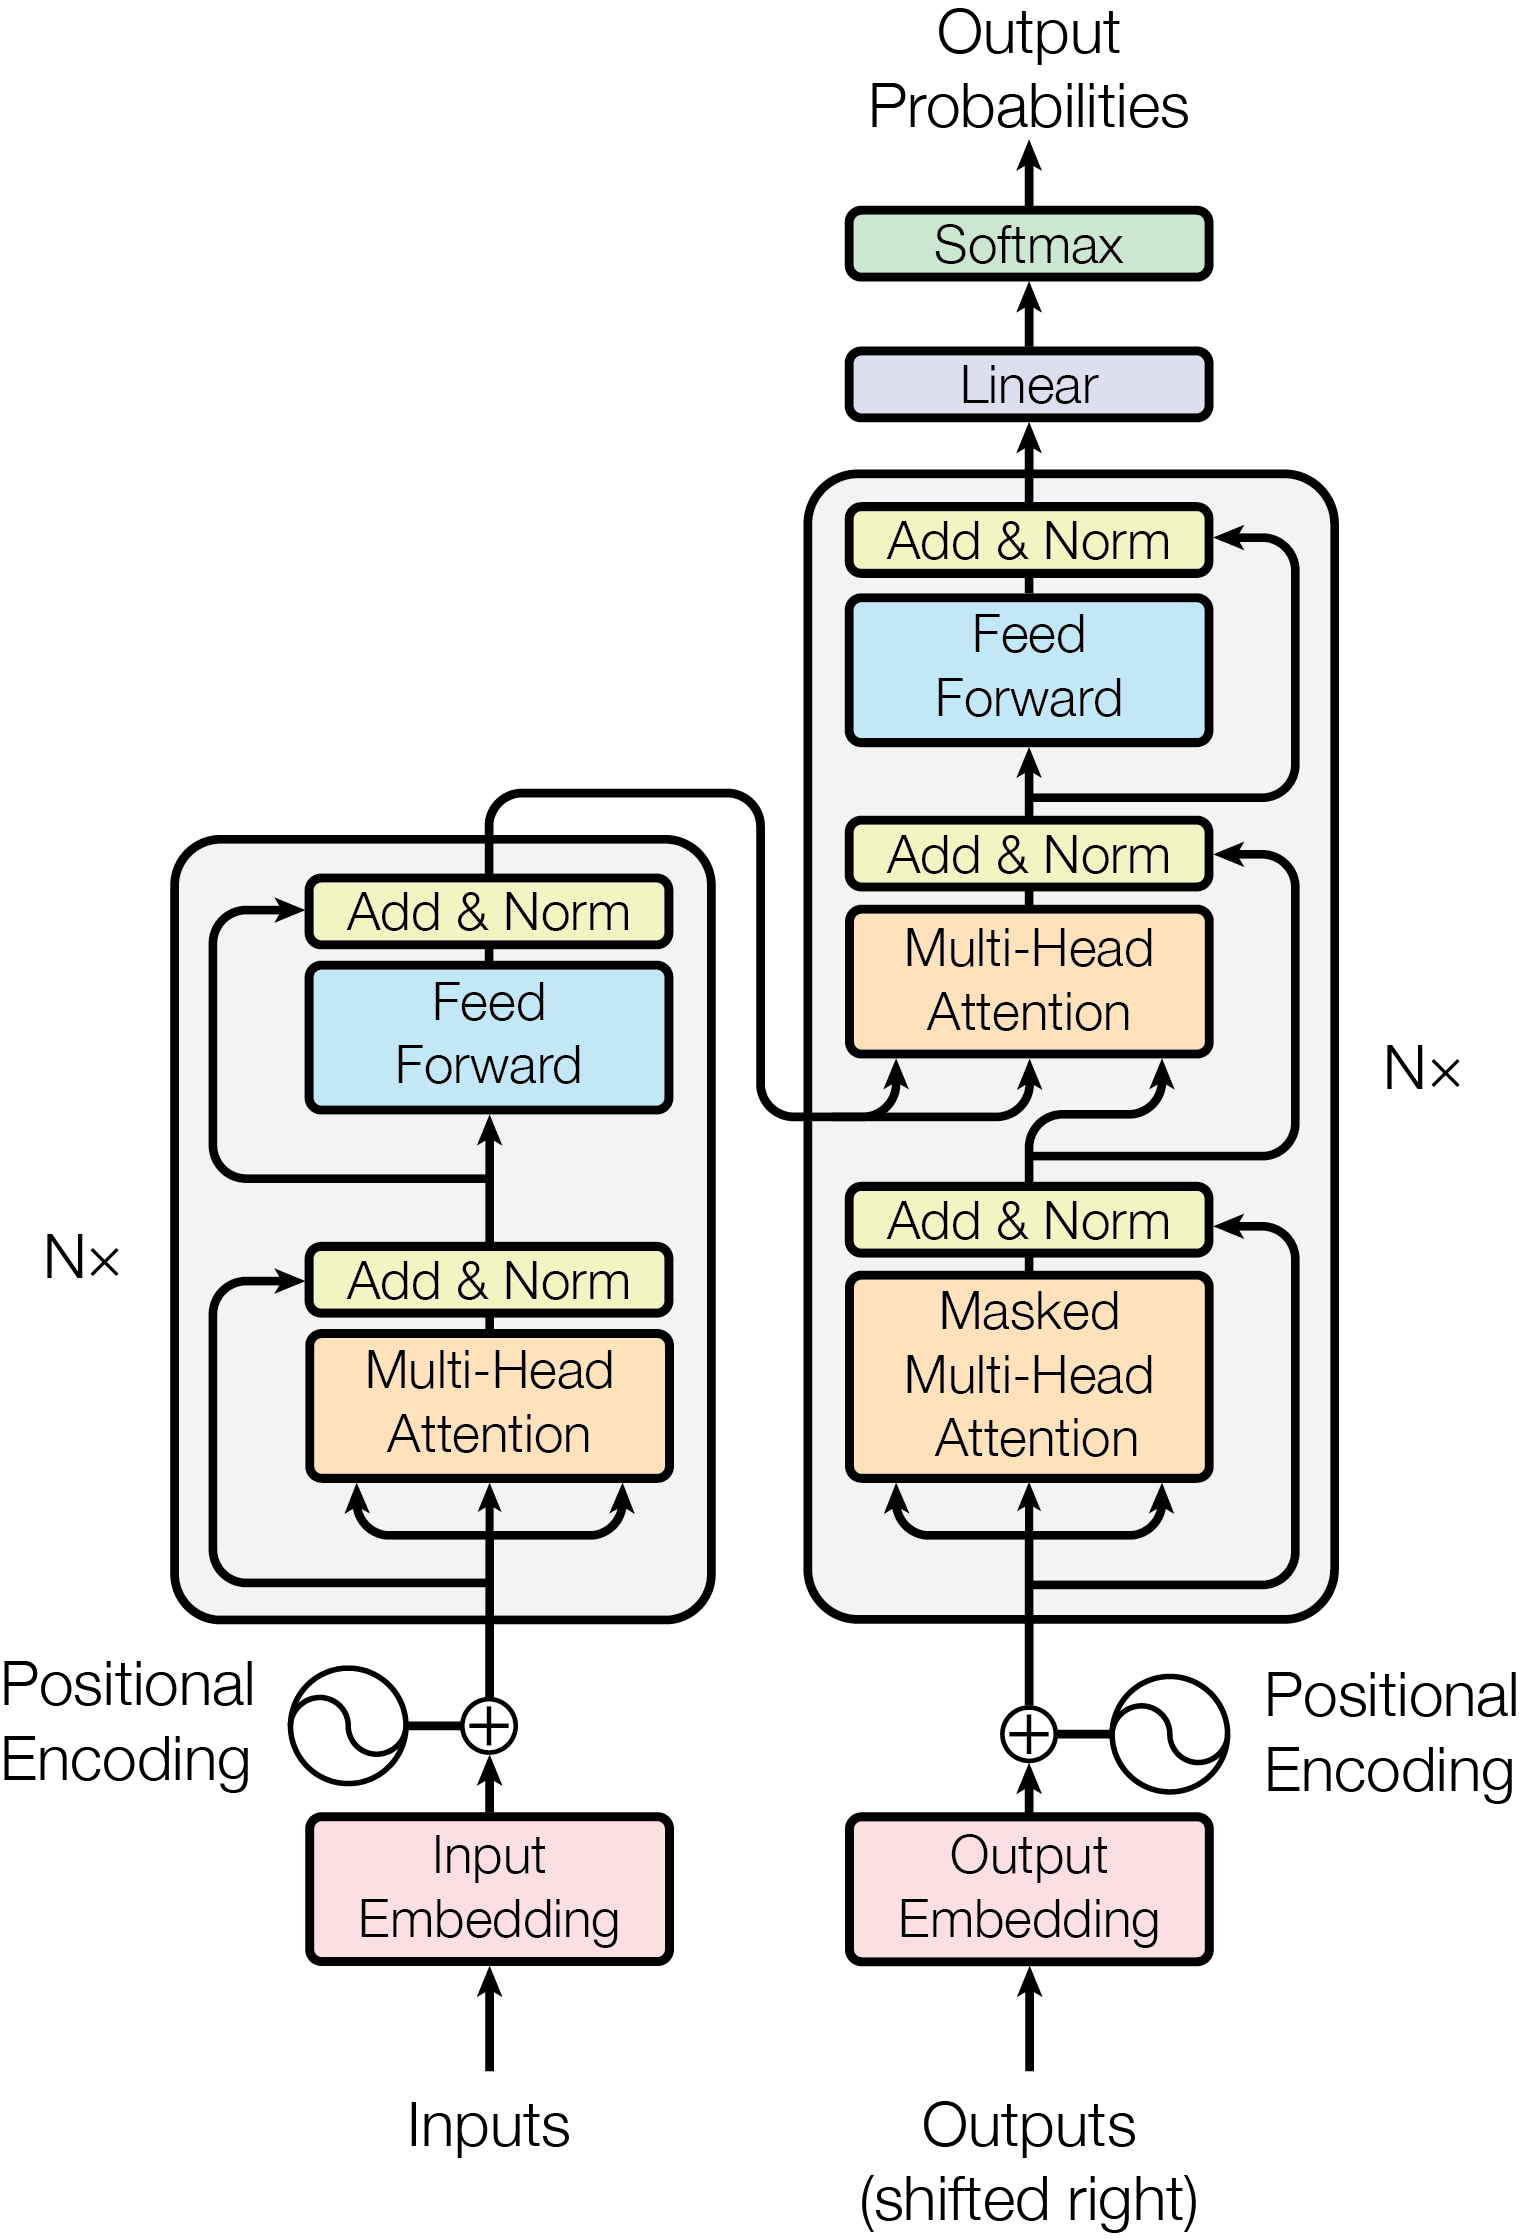
\includegraphics[width=0.5\linewidth]{gambar/ModalNet-21.png}
    \caption{Arsitektur Transformer}
    \label{fig:transformer}
\end{figure}

\subsection{\textit{Positional Encoding}}
Arsitektur Transformer bersifat paralel sehingga diperlukan \textit{Positional Encoding} untuk memberikan informasi urutan pada \textit{sequence}. \textit{Positional Encoding} memiliki ukuran dimensi yang sama dengan \textit{embedding} input sehingga dapat dijumlahkan. Positional encoding dijelaskan pada \ref{subsubsec:pos_enc_sin} dan \ref{subsubsec:trainable_embedding}.

\subsubsection{\textit{Positional encoding sinusoidal}}
\label{subsubsec:pos_enc_sin}
\begin{equation}
    PE_{(pos, 2i)} = \sin \left(pos / 10000^{2i/d_{\text{model}}}\right)
    \label{eq:1}
\end{equation}
\begin{equation}
    PE_{(pos, 2i+1)} = \cos \left(pos / 10000^{2i/d_{\text{model}}}\right)
    \label{eq:2}
\end{equation}

Keterangan:
\begin{itemize}
    \item $PE_{(pos, 2i)}$ adalah posisi pada indeks ganjil
    \item $PE_{(pos, 2i+1)}$ adalah posisi pada indeks genap
    \item $pos$ adalah posisi sampel/data dalan \textit{sequence}
    \item $i$ adalah dimensi data
    \item $d_{\text{model}}$ adalah ukuran embedding
\end{itemize}
$pos$ merupakan posisi dan $i$ merupakan dimensi. $2i$ dan $2i+1$ adalah indeks ganjil dan genap dalam embedding. \textit{Positional encoding sinusoidal} dipilih karena memungkinkan model untuk mengekstrapolasi \textit{sequnece} yang lebih panjang daripada yang ditemui selama pelatihan.

\subsubsection{Trainable Embedding}
\label{subsubsec:trainable_embedding}
\textit{Trainable Embedding} banyak digunakan pada \textit{Large Language Model} (LLM) seperti BERT \cite{devlin2019bertpretrainingdeepbidirectional} dan GPT \cite{radford2019language}. \textit{Trainable Embedding} dapat memahami konteks data lebih baik karena nilainya di-update selama proses pelatihan. Pemahaman kontekstual ini membuat \textit{Trainable embedding} jauh lebih optimal dalam tugas-tugas Deep Learning yang kompleks karena dapat memahami pola yang mungkin terlewatkan oleh \textit{Embedding Statis}.

\subsection{\textit{Attention Mechanism}}
Fungsi \textit{Attention} dapat dideskripsikan sebagai pemetaan \textit{Query} dan sekumpulan pasangan \textit{Key-Value} ke suatu \textit{Output}, di mana \textit{Query}, \textit{Key}, \textit{Value}, dan \textit{Output} semuanya merupakan vektor. \textit{Self-Attention} menghubungkan semua posisi dengan jumlah operasi \textit{sequence} yang konstan sehingga mempercepat operasi dibandingkan layer recurrent pada RNN. Fungsi \textit{Attention} dijelaskan pada persamaan \ref{eq:attention}
% Requires: \usepackage{amsmath}
\begin{equation}
    \text{Attention}(Q, K, V) = \text{softmax}\left(\frac{QK^T}{\sqrt{Head\_DIM}}\right)V
    \label{eq:attention}
\end{equation}
Keterangan:
\begin{itemize}
    \item $\text{Attention}(Q, K, V)$ adalah mekanisme \textit{self-attention}
    \item $Q$ adalah \textit{Query}
    \item $K$ adalah \textit{Key}
    \item $V$ adalah \textit{Value}
    \item $Head\_DIM$ adalah dimensi embedding
\end{itemize}

\textit{Multi-Head Attention} memungkinkan model untuk secara bersamaan memberikan \textit{Attention} informasi dari subruang representasi yang berbeda pada posisi yang berbeda \ref{eq:multi_head_attention}.

\begin{equation}
\begin{aligned}
    \text{MultiHead}(Q, K, V) &= \text{concat}(\text{head}_1, \ldots, \text{head}_h) W^O \\
    \text{dengan head}_i &= \text{Attention}(Q W^Q_i, K W^K_i, V W^V_i)
\end{aligned}
\label{eq:multi_head_attention}
\end{equation}
Keterangan:
\begin{itemize}
    \item $\text{MultiHead}(Q, K, V)$ adalah mekanisme multi-head attention
    \item $\text{head}_i$ adalah mekanisme attention
    \item $W^Q_i$ adalah bobot untuk \textit{Query}
    \item $W^K_i$ adalah bobot untuk \textit{Key}
    \item $W^V_i$ adalah bobot untuk \textit{Value}
    \item $W^O$ adalah bobot untuk multi-head attention
\end{itemize}

\subsection{\textit{Position-wise Feed-Forward Networks}}
Masing-masing lapisan dalam encoder dan decoder terdapat \textit{Feed-Forward Networks} yang saling terhubung, yang diterapkan ke setiap posisi secara terpisah dan identik. Fungsi \textit{Feed-Forward Networks} dapat dilihat pada persamaan \ref{eq:ffn}.

\begin{equation}
   \text{FFN}(x) = \max(0, xW_1 + b_1)W_2 + b_2
   \label{eq:ffn}
\end{equation}
Keterangan:
\begin{itemize}
    \item $\text{FFN}(x)$ adalah mekanisme Feed-Forward Networks
    \item $x$ adalah nilai input neuron
    \item $W_1$ adalah bobot pertama
    \item $b_1$ adalah bias pertama
    \item $W_2$ adalah bobot kedua
    \item $b_2$ adalah bobot kedua
\end{itemize}

Meskipun transformasi linier sama di berbagai posisi, FNN menggunakan parameter yang berbeda pada setiap lapisan.
\subsection{\textit{Layer Nornalization}}
\textit{Layer Normalization} digunakan untuk menormalkan output dari setiap jaringan, sehingga distribusi nilainya stabil selama \textit{training} \ref{eq:layer_normalization}. Parameter $\gamma$ dan $\beta$ merupakan parameter pelatihan dan $\epsilon$ merupakan nilai konstan $10^{-6}$.
\begin{equation}
    \text{LayerNorm}(x) = \frac{x - \mu}{\sqrt{\sigma^2 + \epsilon}} \cdot \gamma + \beta
    \label{eq:layer_normalization}
\end{equation}
Keterangan:
\begin{itemize}
    \item $\text{LayerNorm}(x)$ adalah Layer Normalisasi
    \item $x$ adalah nilai input layer
    \item $\mu$ adalah rataan
    \item $\sigma^2$ adalah standar deviasi
    \item $\epsilon$ adalah nilai galat agar pembagi tidak bernilai $0$
    \item $\gamma \text{ dan } \beta$ adalah parameter pelatihan
\end{itemize}
% Vision Transformer
\section{\textit{Video Vision Transformer}}
Pada ViViT, video input $V$ dengan dimensi $D$ (depth), $H$ (tinggi), $W$ (lebar), dan $C$ (channel) dibagi-bagi menjadi potongan-potongan kecil yang disebut \textit{patch}\cite{arnab2021vivitvideovisiontransformer}. Setiap \textit{patch} $P$ memiliki dimensi $P_d \times P_h \times P_w \times C$.
Proses pembagian video menjadi \textit{patch} ini dapat divisualisasikan sebagai persamaan \ref{eq:reshape}
\begin{equation}
   V \in \mathbb{R}^{D \times H \times W \times C} \rightarrow \text{Reshape} \rightarrow P \in \mathbb{R}^{N \times (P_d \times P_h \times P_w \times C)}
   \label{eq:reshape}
\end{equation}
Keterangan:
\begin{itemize}
    \item $V$ adalah input embedding video
    \item $P$ adalah input patch embedding
    \item $\text{Reshape}$ adalah mengubah input video ke patch
    \item $D$ adalah ukuran \textit{depth} kedalaman/frame
    \item $H$ adalah ukuran \textit{height} atau tinggi
    \item $W$ adalah ukuran \textit{width} atau lebar
    \item $C$ adalah jumlah $channel$ atau kanal
\end{itemize}

di mana $N = (D/P_d) \times (H/P_h) \times (W/P_w)$ adalah jumlah total \textit{patch} yang dihasilkan.
Selanjutnya, setiap \textit{patch} $P$ diproyeksikan ke dalam ruang \textit{embedding} dengan dimensi $d$ melalui sebuah lapisan linear. Hasil proyeksi ini membentuk sebuah \textit{sequence} token $Z$ dengan dimensi $N \times d$ sesuai persamaan \ref{eq:linear_map}
\begin{equation}
    Z = \text{Linear}(P) \in \mathbb{R}^{N \times d} \label{eq:linear_map}
\end{equation}
Keterangan:
\begin{itemize}
    \item $Z$ adalah hasil proyeksi \textit{patch embedding}
    \item $P$ adalah \textit{patch embedding}
\end{itemize}

\textit{Sequence} token $Z$ ditambahkan dengan \textit{positional encoding} yang  kemudian menjadi input untuk \textit{encoder transformer}. Terdapat dua metode utama untuk menghasilkan \textit{patch embedding} yaitu, \textit{Uniform Frame Sampling} yang hanya memiliki informasi spasial dan \textit{Tubelet Embedding} yang menghasilkan \textit{patch} yang mencakup informasi spasial dan temporal.